\section{Versuchsdurchführung}
	\subsection{Messung spektraler Transparenz und Reflexion} \label{sec:shimadzu}
	%TODO: Kurze Beschreibung der Durchführung am SHIMADZU3100 (da reichen ein paar wenige Sätze)
	
	\subsection{Lumineszenzspektrometrie} \label{sec:fluoromax}
	%TODO Kurze Beschreibung der Messung am FLOUROMAX. Besonders  Bragg-Bedingung am Eingangsfilter diskutieren.
	Die Messung der spektralen Verteilung des emittierten Fluoreszenzlichtes einer Probe wird im FLOUROMAX-Lumineszenzspektrometer vorgenommen. Dabei wird eine Probe mit einer ausgewählten Wellenlänge angeregt und es wird mit einem Detektor die Intensitätsverteilung des emittierten Lichtes gemessen. Zum Ausfiltern der entsprechenden Wellenlängen (sowohl des einfallenden, als auch des ausfallenden Lichtes) werden 2 Monochromatoren verwendet. Diese bestehen aus optischen Gittern mit Gitterkonstante $d$, die in einem bestimmten Winkel $\theta$ platziert werden, so dass die gewünschte konstruktive Interferenzbedinung für $m \in \mathbb{Z}$ erfüllt ist:
	\begin{equation} \label{eq:gitter}
		m \cdot \lambda \overset{!}{=} d \cdot \sin\theta.
	\end{equation}
	Zu Beginn wurde die Funktionstüchtigkeit des Monochromators überprüft, indem bei geöffneter Klappe ein weißes Blatt Papier in den Strahlengang gehalten wurde und anhand der Farbe die Richtigkeit der herausgefilterten Wellenlänge geprüft wurde. Dabei fällt auf, dass bereits im normalerweise für das menschliche Auge nicht sichtbare UV-Bereich ein grün-blauer, und somit langwelligerer, Lichtfleck erscheint. Dies kann mit der freien Wahl von $m$ in Gleichung (\ref{eq:gitter}) bei konstanter rechter Seite erklärt werden. Dieses Phänomen trat insbesondere auch bei der Messung des Emissionsspektrums der in Abschnitt \ref{sec:organisch} beschriebenen Farbstoffaufdampfschicht unter Bestrahlung mit Licht der Wellenlänge \unit[280]{nm} auf. Der rote Graph in Abbildung \ref{fig:flouromax_filter} zeigt einen deutlichen Peak bei $\lambda = \unit[560]{nm} = 2\cdot \unit[280]{nm}$. Der Monochromator am Eingang der Messkammer lässt wegen \eqref{eq:gitter} sowohl \unit[280]{nm} als auch \unit[560]{nm} konstruktiv interferieren, wodurch am Ausgang nach entsprechender Transmission durch die Probe der störende Peak entsteht. Diese kann beseitigt werden, indem man am Eingang einen Kantenfilter (Bezeichnung: WG320) verwendet, der Wellenlängen unterhalb einer gewissen Grenzwellenlänge absorbiert. Das so korrigierte Spektrum entspricht dem blauen Graph in Abbildung \ref{fig:flouromax_filter}. Da der Filter auch ein gewisses Absorptionsvermögen in anderen Wellenlängenbereichen hat entsteht weiterhin eine leichte Abschwächung des Signals.
	\begin{figure}
		\centering
		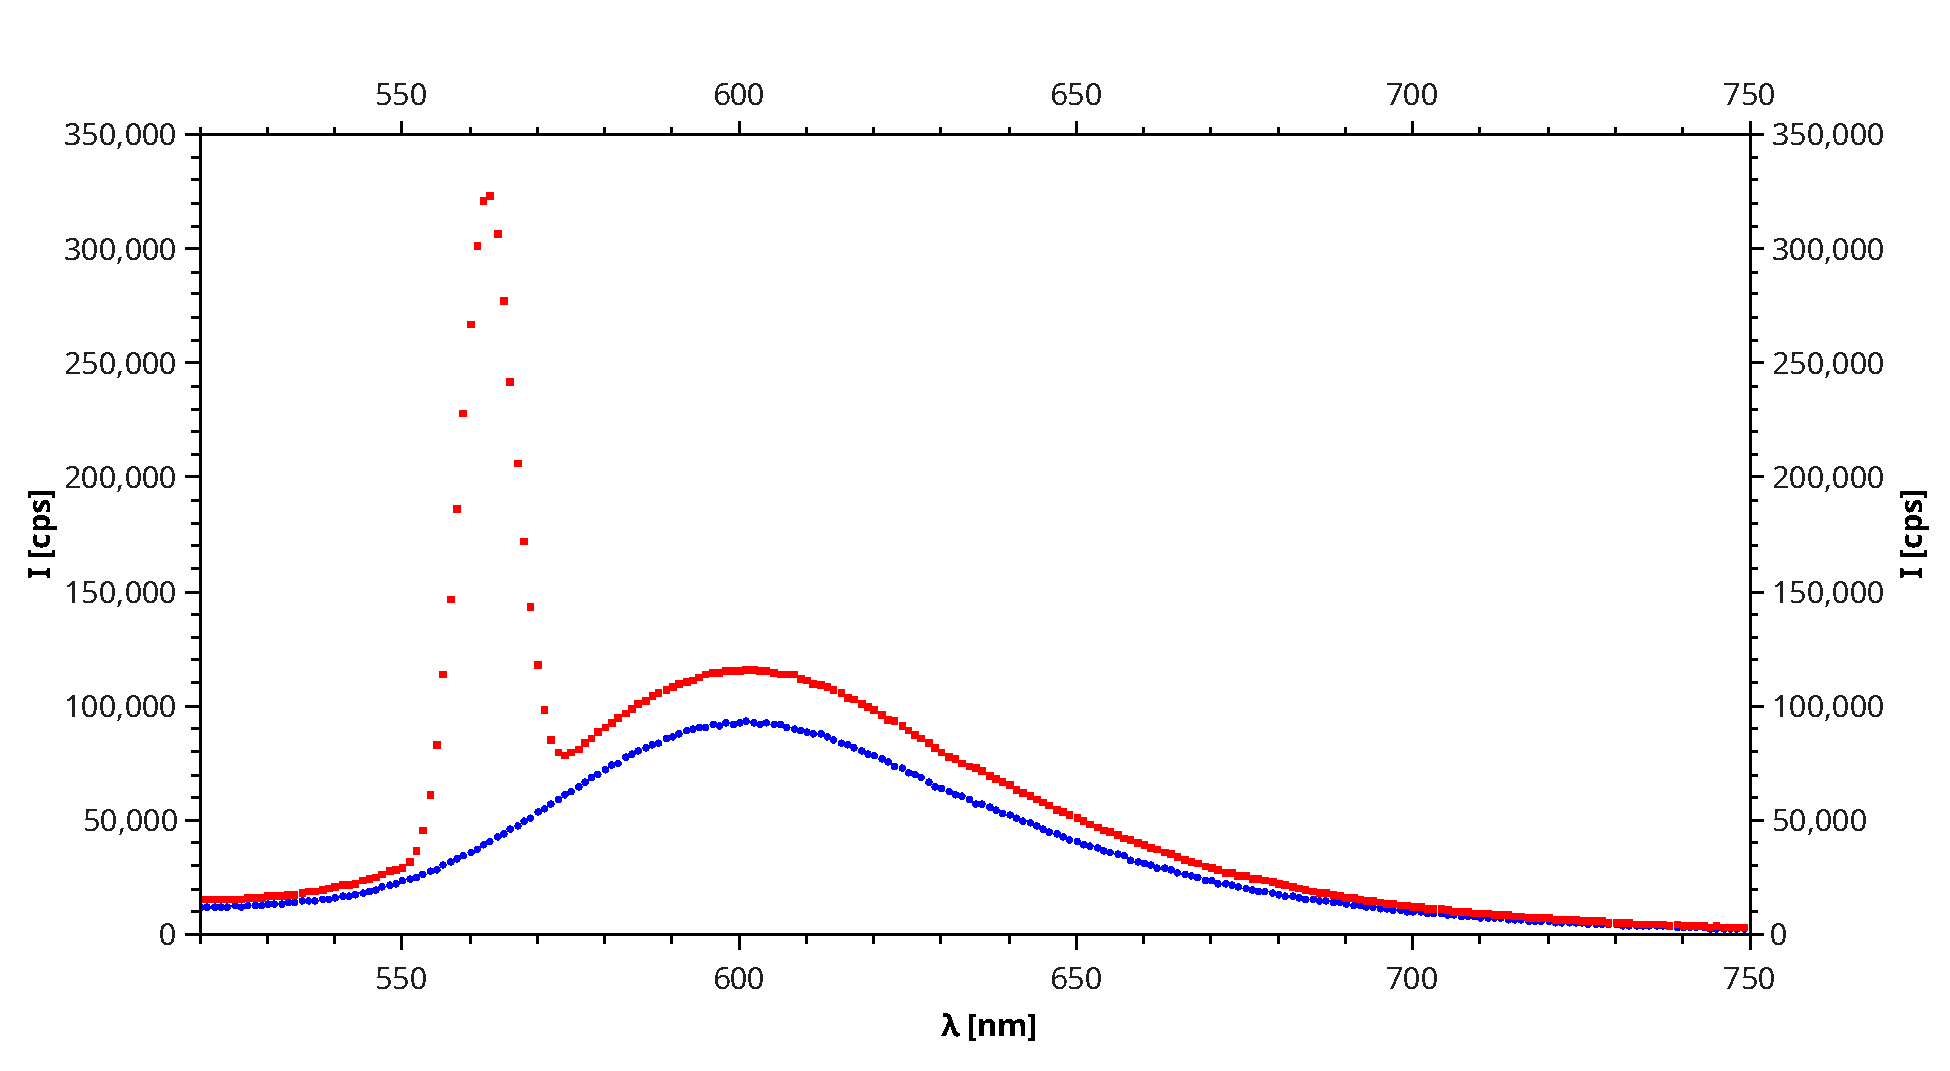
\includegraphics[width=\linewidth]{pic/flouromax_filter}
		\caption{Emissionsspektrum der Farbstoffaufdampfschicht ohne (rot) und mit geeignetem Filter (blau).}
		\label{fig:flouromax_filter}
	\end{figure}